\documentclass[11pt]{article}
\usepackage{myz310e-notes}
\hypersetup{pdftitle={Probability distributions and the Gaussian},pdfauthor={Emre Onur Kahya},pdfsubject={MYZ 310E Machine Learning in Physics, Fall 2026, lecture note 2 (week 1)}}

\AddToHook{env/algorithmic/begin}{\small}
% keep a short box from being split: break the page first if fewer than #1 lines remain
\makeatletter
\newcommand{\keeplines}[1]{\par\penalty-100\begingroup\dimen@=#1\baselineskip\dimen@ii=\pagegoal
  \advance\dimen@ii-\pagetotal\ifdim\dimen@>\dimen@ii\ifdim\dimen@ii>\z@\vfil\fi\break\fi\endgroup}
\makeatother

\begin{document}
\NoteTitle{2}{1}{Probability distributions\\ and the Gaussian}{Probability and Gaussians}{%
Every method in this course either estimates a probability distribution or makes predictions that are best
understood through one. This note collects the probability we need --- how distributions are described, the four
things we do with them, and the multivariate Gaussian in detail --- and connects it to two pillars of modern
machine learning: maximum-likelihood training of language models and Gaussian noise in diffusion models. Every
formula is worked through with small numbers, the derivations are shown step by step, and each algorithm is given
as pseudocode with its running time. Notation follows Note~1, Section~2.}

\section{Describing a distribution}\label{sec:describe}

A random variable $X$ is described by how its probability is spread over its possible values. Three descriptions
are in common use, plus a fourth, empirical one built from data.

\paragraph{Cumulative distribution function} For a real-valued $X$ (integer-valued ones included), the c.d.f.\ is $F(x) = P(X \le x)$. It is
non-decreasing, tends to $0$ as $x \to -\infty$ and to $1$ as $x \to +\infty$, and it exists for every random
variable, discrete or continuous. Probabilities of intervals follow from it, $P(a < X \le b) = F(b) - F(a)$. For a
vector $\X = (X_1, \dots, X_d)$ the inequality is read component-wise:
$F(\x) = P(X_1 \le x_1, \dots, X_d \le x_d)$. The definition needs ordered values. For unordered categories, such as
particle types or text tokens, one first fixes an arbitrary order; Section~\ref{sec:catsample} shows that sampling
with the resulting c.d.f.\ is correct whatever order is chosen.

\paragraph{Probability table (discrete variables)} If $X$ takes finitely or countably many values, its distribution
is the list of probabilities $P(X = x)$, which are non-negative and sum to one. For several discrete variables the
table becomes an array with one axis per variable; a joint table for $d$ variables with $m$ values each has $m^d$
entries --- a first sign of the difficulty Note~3 studies.

\paragraph{Density (continuous variables)} If $F$ is differentiable, the probability density function is
$p(x) = F'(x)$; in $d$ dimensions $p(\x) = \partial^d F/\partial x_1 \cdots \partial x_d$. Probabilities of
regions are integrals,
\[
  P(\X \in A) = \int_A p(\x)\, d\x, \qquad \int_{\R^d} p(\x)\,d\x = 1 .
\]
A density is not a probability: it carries units of $1/[x]$ and may exceed one. Only $p(x)\,\Delta x$, for a small
interval $\Delta x$, is a probability. A Gaussian of width $\sigma = 0.1$~mm has a peak density of about
$4\ \mathrm{mm}^{-1}$, yet the probability of landing in any interval of width $0.01$~mm is at most $0.04$.

\paragraph{The empirical distribution} Given a sample $x_1, \dots, x_n$, the empirical c.d.f.\
$\hat F(x) = \frac{1}{n}\#\{i : x_i \le x\}$ is a step function that jumps by $1/n$ at each data point (by $k/n$ at a
value that occurs $k$ times). For the five measurements $4, 7, 5, 9, 5$ of Section~\ref{sec:mle1d}, $\hat F(3.9) = 0$,
$\hat F(4) = 1/5$, $\hat F(5) = \hat F(6.5) = 3/5$ (a jump of $2/5$ at the repeated value $5$) and $\hat F(9) = 1$. By the law
of large numbers $\hat F(x) \to F(x)$ for every $x$; the convergence is even uniform in $x$ (Glivenko--Cantelli).
The empirical distribution is the simplest estimate of a distribution, and most of the estimators in this course
can be viewed as ways of smoothing it. To evaluate $\hat F$ at many points, sort the sample once ($O(n\log n)$)
and locate each query by binary search ($O(\log n)$ per query, $O(n)$ memory), the same search as in
Section~\ref{sec:catsample}.

\subsection{Joint, marginal and conditional}\label{sec:joint}

For two variables with joint density $p(\x, \vect{z})$ (sums replace integrals in the discrete case):
\begin{align*}
  \text{marginal:} \quad & p(\x) = \int p(\x, \vect{z})\, d\vect{z}, \\
  \text{conditional:} \quad & p(\vect{z} \mid \x) = \frac{p(\x, \vect{z})}{p(\x)} \qquad (p(\x) > 0), \\
  \text{Bayes' rule:} \quad & p(\vect{z} \mid \x) = \frac{p(\x \mid \vect{z})\, p(\vect{z})}{\int p(\x \mid \vect{z}')\, p(\vect{z}')\, d\vect{z}'} .
\end{align*}
Bayes' rule is not a new axiom. The definition of the conditional writes the joint in two ways, the \emph{product
rule} $p(\x, \vect{z}) = p(\vect{z} \mid \x)\,p(\x) = p(\x \mid \vect{z})\,p(\vect{z})$. Dividing both sides by $p(\x)$
gives $p(\vect{z} \mid \x) = p(\x \mid \vect{z})\,p(\vect{z})/p(\x)$, and writing $p(\x)$ as the marginal of the joint,
$p(\x) = \int p(\x \mid \vect{z}')\,p(\vect{z}')\,d\vect{z}'$, gives the denominator.
Independence means $p(\x, \vect{z}) = p(\x)\,p(\vect{z})$, equivalently $p(\vect{z} \mid \x) = p(\vect{z})$.

\begin{worked}{a joint table of two detector flags}
\begin{minipage}[c]{0.5\linewidth}
Two trigger flags fire or not on each recorded event: $A = 1$ if the calorimeter fires, $B = 1$ if the muon chambers
fire. Suppose their joint table is the one on the right, with the marginals in the margins.
\end{minipage}\hfill
\begin{minipage}[c]{0.46\linewidth}\centering\small
\begin{tabular}{@{}lccc@{}}\toprule
 & $B = 0$ & $B = 1$ & $P(A)$ \\ \midrule
$A = 0$ & $0.50$ & $0.10$ & $0.60$ \\
$A = 1$ & $0.15$ & $0.25$ & $0.40$ \\ \midrule
$P(B)$ & $0.65$ & $0.35$ & $1$ \\ \bottomrule
\end{tabular}
\end{minipage}\par\smallskip
\emph{Marginals} are row and column sums: $P(A = 1) = 0.15 + 0.25 = 0.40$ and $P(B = 1) = 0.10 + 0.25 = 0.35$.
\emph{Conditionals} renormalise one row: $P(B = 1 \mid A = 1) = 0.25 / 0.40 = 0.625$, while $P(B = 1 \mid A = 0) =
0.10/0.60 \approx 0.167$. Knowing that the calorimeter fired raises the probability of a muon-chamber signal from
$0.35$ to $0.625$, so the flags are \emph{not} independent; equivalently, $P(A = 1)\,P(B = 1) = 0.14 \ne 0.25 =
P(A = 1, B = 1)$.
\end{worked}

\begin{worked}{Bayes' rule for particle identification}
In a sample of charged tracks, 10\% are kaons and 90\% pions. A particle-identification algorithm tags a true kaon
with probability $0.90$ (its efficiency) and wrongly tags a pion with probability $0.05$ (its mis-identification
rate). What fraction of tagged tracks are kaons? With $K$ = ``is a kaon'' and $T$ = ``is tagged'',
\[
  P(K \mid T) = \frac{P(T \mid K)\,P(K)}{P(T \mid K)\,P(K) + P(T \mid \bar K)\,P(\bar K)}
  = \frac{0.90 \times 0.10}{0.90 \times 0.10 + 0.05 \times 0.90} = \frac{0.090}{0.135} \approx 0.67 .
\]
Although the tagger is right 90\% of the time on kaons, one tagged track in three is a pion, because pions are nine
times more common. The prior $P(K)$ matters as much as the likelihood $P(T \mid K)$; Note~6 builds classifiers on
exactly this computation.
\end{worked}

\subsection{Expectation, variance and covariance}\label{sec:moments}

Expectations are integrals against the density, $\E[g(\X)] = \int g(\x)\,p(\x)\,d\x$ (a sum for discrete
variables). The mean is $\vmu = \E[\X]$, and the covariance matrix is
\[
  \Sigma = \Cov(\X) = \E\big[(\X - \vmu)(\X - \vmu)\T\big], \qquad \Sigma_{jk} = \E[(X_j - \mu_j)(X_k - \mu_k)],
\]
with the variances $\Var(X_j) = \Sigma_{jj}$ on its diagonal. The \emph{correlation coefficient}
$\rho_{jk} = \Sigma_{jk}/\sqrt{\Sigma_{jj}\Sigma_{kk}}$ lies in $[-1, 1]$ and measures linear dependence only.
Three rules are used throughout the course. The first is linearity, $\E[A\X + \vect{b}] = A\,\E[\X] + \vect{b}$ for
a fixed matrix $A$ and vector $\vect{b}$, because an integral is linear. Expanding the product in the definition
and using linearity gives the useful shortcuts $\Var(X) = \E[X^2] - (\E[X])^2$ and $\Cov(X, Z) = \E[XZ] -
\E[X]\,\E[Z]$. The second is how a covariance changes under a
linear map. Let $\vect{Y} = A\X + \vect{b}$. Then, step by step,
\begin{align*}
  \vect{Y} - \E[\vect{Y}] &= A\X + \vect{b} - (A\vmu + \vect{b}) = A(\X - \vmu), \\
  \Cov(\vect{Y}) &= \E\big[A(\X - \vmu)\,(A(\X - \vmu))\T\big] = \E\big[A(\X - \vmu)(\X - \vmu)\T A\T\big]
  = A\,\E\big[(\X - \vmu)(\X - \vmu)\T\big]\,A\T,
\end{align*}
so
\begin{equation}\label{eq:covlin}
  \Cov(A\X + \vect{b}) = A\,\Sigma\,A\T .
\end{equation}
In one dimension this is the familiar $\Var(aX + b) = a^2\Var(X)$: a shift does not change the spread and a scale
multiplies it by $a^2$. The third rule follows from \eqref{eq:covlin} with $A = \vect{v}\T$ a single row: for any
$\vect{v}$, $\Var(\vect{v}\T\X) = \vect{v}\T\Sigma\vect{v} \ge 0$. A covariance matrix is therefore symmetric and
\emph{positive semi-definite}; it is positive definite unless some combination $\vect{v}\T\X$ is constant. Finally,
independent variables are uncorrelated, but uncorrelated variables need not be independent: if $X$ is uniform on
$[-1, 1]$ and $Z = X^2$, then $\E[X] = 0$ and $\Cov(X, Z) = \E[XZ] - \E[X]\,\E[Z] = \E[X^3] = 0$, because $x^3$ is
odd and $X$ is symmetric about $0$; yet $Z$ is a function of $X$.

\section{Four things we do with a distribution}\label{sec:operations}

Whether the distribution is a probability table, a Gaussian or a neural network with billions of parameters, the
same four operations recur.

\begin{enumerate}
\item \textbf{Sample}: generate new data $\x \sim p$. This is what a generative model is for.
\item \textbf{Evaluate}: compute $p(\x)$, the density (or probability) the model assigns to an observation,
summing or integrating out anything that was not recorded. Viewed as a function of the model parameters for fixed
data, the same number is called the \emph{likelihood}. Low likelihood flags unusual data.
\item \textbf{Infer}: predict the hidden part of a configuration from the observed part, for example by its single
most likely value or by its average $\E[\vect{Z} \mid \X = \x]$. Supervised learning is inference of $Y$ from $\X$.
\item \textbf{Learn}: choose the parameters $\theta$ of a family $p_\theta$ from data. The standard principle is
\emph{maximum likelihood},
\begin{equation}\label{eq:mle}
  \hat\theta = \argmax_\theta \prod_{i=1}^n p_\theta(\x_i) = \argmin_\theta \; -\frac{1}{n}\sum_{i=1}^n \log p_\theta(\x_i),
\end{equation}
the product being justified by the i.i.d.\ assumption. Taking the logarithm changes nothing about the maximiser,
because $\log$ is increasing, but turns a product of $n$ small numbers (which underflows) into a sum (which does
not) and makes derivatives easy. The right-hand side is the average negative log-likelihood, the density-estimation
loss of Note~1, Table~2.
\end{enumerate}

\begin{worked}{a categorical distribution learned from counts}
The number $X \in \{0, 1, 2\}$ of reconstructed jets in a simplified event selection is described by three numbers
$\pi_0, \pi_1, \pi_2 \ge 0$ with $\sum_k \pi_k = 1$ --- a \emph{categorical} distribution with $m = 3$ categories.
In $n = 50$ selected events we count $n_0 = 12$, $n_1 = 30$, $n_2 = 8$.
\begin{itemize}
\item \emph{Learn.} Maximum likelihood gives the observed frequencies (derived in Section~\ref{sec:catmle}):
$\hat\pi_0 = 12/50 = 0.24$, $\hat\pi_1 = 30/50 = 0.60$, $\hat\pi_2 = 8/50 = 0.16$ (Figure~\ref{fig:categorical},
left).
\item \emph{Evaluate.} The log-likelihood of the data is $\sum_k n_k \log\hat\pi_k = 12\log 0.24 + 30\log 0.60 +
8\log 0.16 \approx -47.11$, i.e.\ an average negative log-likelihood of $0.942$ nats per event (nats are natural-logarithm units; dividing by
$\ln 2$ gives bits). The uniform guess
$\pi_k = 1/3$ gives $50\log(1/3) \approx -54.93$: the fitted model explains the data better, as it must.
\item \emph{Sample.} The c.d.f.\ is $F(0) = 0.24$, $F(1) = 0.84$, $F(2) = 1$. Draw $u$ uniform on $[0, 1)$ and
return the first $k$ with $F(k) > u$: $u = 0.10$ gives $k = 0$, $u = 0.55$ gives $k = 1$ and $u = 0.90$ gives $k = 2$
(Figure~\ref{fig:categorical}, right). Each $k$ is returned with probability equal to the length of its step,
$\hat\pi_k$.
\item \emph{Infer.} The most probable multiplicity is $1$, and the mean is $0 \times 0.24 + 1 \times 0.60 + 2 \times
0.16 = 0.92$ jets.
\end{itemize}
\end{worked}

\begin{figure}[htbp]
\centering
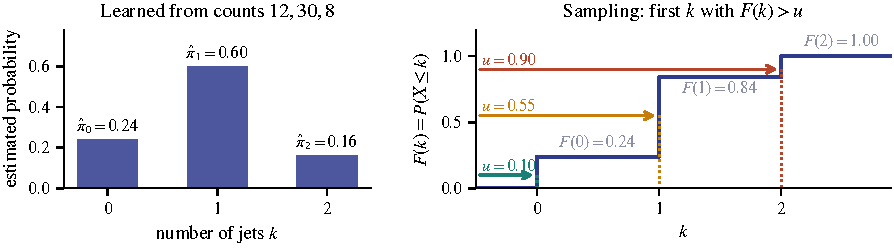
\includegraphics[width=0.84\linewidth]{figures/n2_categorical.pdf}
\caption{The categorical example. Left: maximum-likelihood probabilities from the counts $12, 30, 8$. Right:
inverse-c.d.f.\ sampling. A uniform $u$ is sent horizontally until it meets the staircase $F$; the step it hits is
the sample.}
\label{fig:categorical}
\end{figure}

\subsection{Maximum likelihood for a categorical distribution}\label{sec:catmle}

With $m$ categories and counts $n_1, \dots, n_m$ ($\sum_k n_k = n$), the probability of the data is
$\prod_i \pi_{x_i} = \prod_k \pi_k^{n_k}$, so the log-likelihood is
\[
  \ell(\pi) = \sum_{k=1}^m n_k \log \pi_k, \qquad \text{to be maximised subject to } \sum_{k=1}^m \pi_k = 1 .
\]
The constraint matters: without it, $\ell$ grows without bound as every $\pi_k$ grows. A constrained maximum is found
with a \emph{Lagrange multiplier} $\lambda$. Form
\[
  \mathcal{L}(\pi, \lambda) = \sum_k n_k \log\pi_k + \lambda\Big(1 - \sum_k \pi_k\Big)
\]
and set its derivatives to zero:
\begin{align*}
  \frac{\partial\mathcal{L}}{\partial\pi_k} = \frac{n_k}{\pi_k} - \lambda = 0
  &\quad\Longrightarrow\quad \pi_k = \frac{n_k}{\lambda} \quad (k = 1, \dots, m), \\
  \frac{\partial\mathcal{L}}{\partial\lambda} = 1 - \sum_k \pi_k = 0
  &\quad\Longrightarrow\quad 1 = \sum_k \frac{n_k}{\lambda} = \frac{n}{\lambda}
  \quad\Longrightarrow\quad \lambda = n .
\end{align*}
Hence
\begin{equation}\label{eq:catmle}
  \hat\pi_k = \frac{n_k}{n} .
\end{equation}
This stationary point is the maximum: each $\log\pi_k$ is concave, so $\ell$ is concave, and a concave function on the
convex set of probability vectors has no other local maxima. In the language of losses, dividing $\ell$ by $n$ gives
$\sum_k \hat p_k \log\pi_k$ with $\hat p_k = n_k/n$, so maximum likelihood minimises the \emph{cross-entropy}
$-\sum_k \hat p_k \log\pi_k$ between the observed frequencies and the model (Note~4, Section~2), and the minimum is
reached when the model reproduces the frequencies.

\paragraph{Zero counts} If a category never occurs, $n_k = 0$ and $\hat\pi_k = 0$: the model declares the category
impossible. A single later occurrence then has log-likelihood $\log 0 = -\infty$. The standard remedy adds a
\emph{pseudo-count} $\alpha > 0$ to every category,
\begin{equation}\label{eq:pseudocount}
  \hat\pi_k^{(\alpha)} = \frac{n_k + \alpha}{n + \alpha m},
\end{equation}
which with $\alpha = 1$ (Laplace smoothing) turns the jet counts into the probabilities $13/53$, $31/53$ and $9/53$,
that is $0.245$, $0.585$ and $0.170$. The correction matters for small $n_k$ and fades as $n$ grows; Note~6, Section~4, uses it in naive Bayes.

\subsection{Sampling from a categorical distribution}\label{sec:catsample}

The sampling rule of the worked example is the \emph{inverse-c.d.f.\ method}. Number the categories $1, \dots, m$
(in the jet example, category $k$ is $k - 1$ jets) and set $F(0) = 0$. If $U$ is uniform on $[0,1)$, the
returned value is $k$ exactly when $F(k-1) \le U < F(k)$, which happens with probability $F(k) - F(k-1) = \pi_k$. For unordered categories the numbering is arbitrary,
and any numbering works, because each step of the staircase still has length $\pi_k$. The same idea samples a
continuous $X$ with an invertible c.d.f.: the variable $F^{-1}(U)$ satisfies $P(F^{-1}(U) \le x) = P(U \le F(x)) = F(x)$, so a draw is $x = F^{-1}(u)$. For
example, the exponential decay-time density $p(x) = e^{-x/\tau}/\tau$ has $F(x) = 1 - e^{-x/\tau}$, so
$x = -\tau\log(1 - u)$.
Scanning the categories one by one costs up to $m$ steps per draw. When many samples are needed from the same
distribution, the cumulative sums can be computed once and the first $k$ with $F(k) > u$ found by \emph{binary
search}, because $F$ is sorted.

\begin{worked}{binary search on a staircase}
Take $m = 8$ categories with cumulative sums $F_{1:8} = (0.05, 0.15, 0.30, 0.40, 0.55, 0.75, 0.90, 1)$ and $u = 0.70$.
\textsc{SampleBinary} of Algorithm~\ref{alg:catsample} starts with $lo = 1$, $hi = 8$.
\begin{center}\small
\begin{tabular}{@{}cccccl@{}}\toprule
Step & $lo$ & $hi$ & $mid$ & $F_{mid}$ & action \\ \midrule
1 & 1 & 8 & 4 & 0.40 & $0.40 \le u$: $lo \gets 5$ \\
2 & 5 & 8 & 6 & 0.75 & $0.75 > u$: $hi \gets 6$ \\
3 & 5 & 6 & 5 & 0.55 & $0.55 \le u$: $lo \gets 6$ \\ \bottomrule
\end{tabular}
\end{center}
Now $lo = hi = 6$, and indeed $F_5 = 0.55 \le 0.70 < 0.75 = F_6$. Three comparisons, $\log_2 8$, where the linear
scan would have needed six.
\end{worked}

\begin{algorithm}[!tb]
\caption{The categorical distribution: fitting by counting; sampling by inverse c.d.f.}\label{alg:catsample}
\begin{algorithmic}[1]
\Require labels $x_1, \dots, x_n \in \{1, \dots, m\}$; pseudo-count $\alpha \ge 0$ ($\alpha = 0$ is maximum likelihood)
\Function{FitCategorical}{$x_{1:n}, m, \alpha$}
  \State $c_k \gets 0$ for $k = 1, \dots, m$
  \For{$i = 1, \dots, n$} $c_{x_i} \gets c_{x_i} + 1$ \Comment{one pass over the data}
  \EndFor
  \State \Return $\hat\pi_k = (c_k + \alpha)/(n + \alpha m)$ for $k = 1, \dots, m$ \Comment{equation \eqref{eq:pseudocount}}
\EndFunction
\Statex \textbf{Sampling} from probabilities $\pi_1, \dots, \pi_m$ (non-negative, sum one):
\Function{SampleLinear}{$\pi$}
  \State draw $u \sim \mathrm{Uniform}[0, 1)$; \ $F \gets 0$ \Comment{running c.d.f.}
  \For{$k = 1, \dots, m$}
    \State $F \gets F + \pi_k$
    \If{$F > u$} \Return $k$ \EndIf
  \EndFor
  \State \Return $m$ \Comment{guards against round-off in $\sum_k \pi_k$}
\EndFunction
\Function{SampleBinary}{$F_{1:m}$} \Comment{$F_k = \pi_1 + \dots + \pi_k$, computed once in $O(m)$}
  \State draw $u \sim \mathrm{Uniform}[0, 1)$; \ $lo \gets 1$; \ $hi \gets m$
  \While{$lo < hi$} \Comment{invariant: the answer lies in $\{lo, \dots, hi\}$}
    \State $mid \gets \lfloor (lo + hi)/2 \rfloor$
    \If{$F_{mid} > u$} $hi \gets mid$ \Else\ $lo \gets mid + 1$ \EndIf
  \EndWhile
  \State \Return $lo$
\EndFunction
\end{algorithmic}
\end{algorithm}

\keeplines{9}
\begin{runtime}{fitting and sampling a categorical distribution}
\emph{Fitting}: $O(n + m)$ time --- one increment per example plus one division per
category --- and $O(m)$ memory for the counts; the data can be streamed and need not be stored.
\emph{Sampling, linear scan}: $O(m)$ per draw in the worst case, $O(1)$ extra memory.
\emph{Sampling, binary search}: $O(m)$ once to build $F$, then $O(\log m)$ per draw, because each step halves the
interval $\{lo, \dots, hi\}$; memory $O(m)$. For $m = 10^5$ (a language-model vocabulary) a draw takes about $17$
comparisons instead of up to $10^5$. The alias method even reaches $O(1)$ per draw after $O(m)$ preparation.
In a language model $\pi$ changes at every token, so producing it (the network, then an $O(m)$ softmax) dominates,
and the $O(m)$ cumulative sum makes binary search pointless for a single draw. (The softmax
normalisation is defined in the box below.)
\end{runtime}

\begin{modern}{a language model is a categorical distribution}
A large language model defines, for every prefix of text, a categorical distribution over a vocabulary of
$V \approx 10^5$ tokens (words or pieces of words). The network outputs one real score per token, the
``logits'' $z_1, \dots, z_V$, and the probabilities are given by the \emph{softmax}
$\pi_k = e^{z_k/T} / \sum_j e^{z_j/T}$, where the \emph{temperature} $T = 1$ during training. All four operations
appear: training is maximum likelihood \eqref{eq:mle} on the next token, i.e.\ minimising cross-entropy; generating
text is repeated sampling (Algorithm~\ref{alg:catsample}), with $T < 1$ concentrating mass on likely tokens,
$T \to 0$ giving the single most probable token and $T \to \infty$ approaching the uniform distribution; evaluating
the likelihood of a text gives its \emph{perplexity}, $\exp$ of the average negative log-likelihood per token; and
answering a question is inference, conditioning on the prompt. The worked example above --- learned frequencies from
counts, with perplexity $e^{0.942} \approx 2.57$ --- is the simplest version of this. Counting next-token frequencies
separately for every possible prefix would repeat that fit once per prefix, but almost every long prefix occurs zero
times in the training text, so counting fails. A neural network instead uses the same weights for all prefixes, so
what it learns from one prefix also informs similar ones.
\end{modern}

\section{The univariate Gaussian}\label{sec:gauss1d}

The Gaussian (normal) density with mean $\mu$ and variance $\sigma^2$ is
\begin{equation}\label{eq:gauss1d}
  \Normal(x; \mu, \sigma^2) = \frac{1}{\sqrt{2\pi\sigma^2}} \exp\!\left( -\frac{(x - \mu)^2}{2\sigma^2} \right).
\end{equation}
It is a symmetric bump centred at $\mu$ with width set by the standard deviation $\sigma$
(Figure~\ref{fig:gauss1d}). About $68.3\%$, $95.4\%$ and $99.7\%$ of the probability lies within one, two and three
standard deviations of the mean; physicists' ``$5\sigma$'' discovery threshold corresponds to a one-sided tail
probability of $2.9 \times 10^{-7}$. Any Gaussian is a shifted and scaled standard one:
$X = \mu + \sigma Z$ with $Z \sim \Normal(0, 1)$.

\noindent\begin{minipage}[c]{0.54\linewidth}\centering
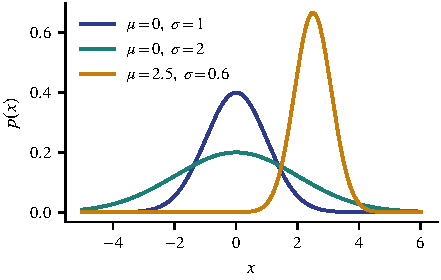
\includegraphics[width=\linewidth]{figures/gaussian_1d.pdf}
\captionof{figure}{Gaussian densities. Doubling $\sigma$ halves the peak height, since the area stays one.}
\label{fig:gauss1d}
\end{minipage}\hfill
\begin{minipage}[c]{0.42\linewidth}
\emph{Why this particular shape.} The central limit theorem says that a sum of many independent contributions with
finite variance is approximately Gaussian, whatever the individual distributions, provided no single contribution
dominates the sum. Measurement noise built from many small effects is therefore often close to Gaussian. A second
reason is that, among all densities with a given mean and variance, the Gaussian has maximal entropy
$H = -\int p\log p\,dx$ (the information-theoretic analogue of the Gibbs entropy): it assumes nothing beyond those
two numbers.
\end{minipage}\par\medskip

\subsection{Standardising and computing probabilities}\label{sec:standardise}

The Gaussian c.d.f.\ cannot be written with elementary functions. Every Gaussian probability is instead reduced to the standard c.d.f.\
$\Phi(z) = P(Z \le z)$ by \emph{standardising}: if $X = \mu + \sigma Z$, then $X \le x$ exactly when
$Z \le (x - \mu)/\sigma$, so
\[
  P(X \le x) = \Phi\!\Big(\frac{x - \mu}{\sigma}\Big), \qquad z = \frac{x - \mu}{\sigma}
  \text{ is the \emph{$z$-score} of } x .
\]
The symmetry of the bump gives $\Phi(-z) = 1 - \Phi(z)$, and a two-sided interval has
$P(\lvert Z\rvert \le z) = 2\Phi(z) - 1$. A handful of values suffices for most purposes:
\begin{center}\small
\begin{tabular}{@{}lcccccccc@{}}\toprule
$z$ & $0$ & $0.5$ & $1$ & $1.5$ & $1.645$ & $1.96$ & $2$ & $3$ \\ \midrule
$\Phi(z)$ & $0.5000$ & $0.6915$ & $0.8413$ & $0.9332$ & $0.9500$ & $0.9750$ & $0.9772$ & $0.9987$ \\
$2\Phi(z) - 1$ & $0$ & $0.383$ & $0.683$ & $0.866$ & $0.900$ & $0.950$ & $0.954$ & $0.997$ \\ \bottomrule
\end{tabular}
\end{center}
The last row is the ``68--95--99.7'' rule, and the columns $1.645$ and $1.96$ give the familiar 90\% and 95\%
intervals.

\begin{worked}{probabilities for a calibrated energy measurement}
Suppose a simple calorimeter measures the energy of $50$~GeV electrons with Gaussian resolution, $X \sim
\Normal(50, 2^2)$ in GeV (a deliberately coarse, hypothetical resolution).
\begin{itemize}
\item $P(X > 54)$: the $z$-score is $(54 - 50)/2 = 2$, so $P = 1 - \Phi(2) = 1 - 0.9772 = 0.0228$. About one
electron in 44 is measured above $54$~GeV.
\item $P(47 < X < 53)$: $z = \pm 1.5$, so $P = 2\Phi(1.5) - 1 = 0.866$.
\item $P(X < 49)$: $z = -0.5$, so $P = \Phi(-0.5) = 1 - 0.6915 = 0.3085$.
\item The interval containing the central 90\% is $50 \pm 1.645 \times 2 = [46.71, 53.29]$~GeV.
\end{itemize}
The peak density is $1/\sqrt{2\pi \cdot 4} \approx 0.199\ \mathrm{GeV}^{-1}$; multiplying by a bin width of
$0.1$~GeV gives the approximate probability $0.020$ of a measurement within $\pm 0.05$~GeV of $50$.
\end{worked}

\subsection{Gaussian noise and squared error}\label{sec:noise}

Suppose targets are generated as $y = f(x) + \varepsilon$ with $\varepsilon \sim \Normal(0, \sigma^2)$, independently
for each example. Then $y \mid x \sim \Normal(f(x), \sigma^2)$ and, taking $-\log$ of \eqref{eq:gauss1d},
\[
  -\log p(y \mid x) = \frac{(y - f(x))^2}{2\sigma^2} + \frac12 \log(2\pi\sigma^2) .
\]
Summed over a dataset, this is $\frac{1}{2\sigma^2}\sum_i (y_i - f(x_i))^2 + \frac{n}{2}\log(2\pi\sigma^2)$. The
second term does not depend on $f$, and the factor $1/(2\sigma^2)$ is a positive constant, so the $f$ that
maximises the likelihood is the $f$ that minimises the sum of squared errors, whatever the value of $\sigma$. The
squared loss of Note~1, Table~2, is maximum likelihood under Gaussian noise; Note~8, Section~2, builds least squares
on this fact, and heavier-tailed noise calls for other losses (Question~C3).

\begin{physics}{$\chi^2$ fits are Gaussian likelihoods}
Fitting a model $f_\theta$ to measurements $y_i \pm \sigma_i$ by minimising $\chi^2 = \sum_i (y_i -
f_\theta(x_i))^2 / \sigma_i^2$ is maximum likelihood with independent Gaussian errors of known widths: the derivation
above with a different $\sigma_i$ for each point gives $-2\log$ likelihood $= \chi^2 + {}$const. The familiar
rule ``$\Delta\chi^2 = 1$ gives the $1\sigma$ interval'' of a single parameter is the statement that $-2\log$ likelihood is quadratic
near its minimum~\cite{cowan1998}. When errors are correlated, the sum becomes the quadratic form of the next
section, with the covariance matrix of the measurements.
\end{physics}

\section{The multivariate Gaussian}\label{sec:gaussnd}

For $\x \in \R^d$, the Gaussian with mean $\vmu \in \R^d$ and symmetric positive-definite covariance matrix
$\Sigma \in \R^{d \times d}$ is
\begin{equation}\label{eq:gaussnd}
  \Normal(\x; \vmu, \Sigma) = \frac{1}{(2\pi)^{d/2} \lvert\Sigma\rvert^{1/2}}
  \exp\!\left( -\tfrac12 (\x - \vmu)\T \Sigma^{-1} (\x - \vmu) \right),
\end{equation}
where $\lvert\Sigma\rvert$ is the determinant. For $d = 1$ it reduces to \eqref{eq:gauss1d}. The prefactor only
normalises the density; all the shape is in the exponent. The quantity
\[
  \Delta^2(\x) = (\x - \vmu)\T \Sigma^{-1} (\x - \vmu)
\]
is the squared \emph{Mahalanobis distance} of $\x$ from the mean: Euclidean distance after the data have been
rotated to the principal axes and rescaled so that every direction has unit variance (``whitened''; see the
eigendecomposition below). Surfaces of constant density are the ellipsoids
$\Delta^2 = \text{const}$. If the components are independent, $\Sigma = \operatorname{diag}(\sigma_1^2, \dots,
\sigma_d^2)$, then $\Delta^2 = \sum_j (x_j - \mu_j)^2/\sigma_j^2$ is a sum of squared $z$-scores and the density is
the product of $d$ one-dimensional Gaussians, $\prod_j \Normal(x_j; \mu_j, \sigma_j^2)$. In the \emph{isotropic} case
$\Sigma = \sigma^2 I$ we have $\lvert\Sigma\rvert = \sigma^{2d}$ and $\Sigma^{-1} = I/\sigma^2$, so
\begin{equation}\label{eq:gaussiso}
  \Normal(\x; \vmu, \sigma^2 I) = \frac{1}{(2\pi\sigma^2)^{d/2}} \exp\!\left( -\frac{\norm{\x - \vmu}^2}{2\sigma^2} \right):
\end{equation}
the Mahalanobis distance is the Euclidean distance divided by $\sigma$, and the contours are spheres. For $d = 2$
and $\sigma = 1$ the peak density is $1/(2\pi) \approx 0.159$.

\paragraph{Linear maps keep a Gaussian Gaussian} A property used repeatedly below: if $\X \sim \Normal(\vmu, \Sigma)$
and $A$ is a fixed $k \times d$ matrix of rank $k$, then
\begin{equation}\label{eq:gausslin}
  A\X + \vect{b} \sim \Normal\big(A\vmu + \vect{b},\; A\Sigma A\T\big).
\end{equation}
The mean and covariance are those of \eqref{eq:covlin}; that the result is again Gaussian follows, for invertible
$A$, from a change of variables in \eqref{eq:gaussnd}, and in general is a standard result~\cite{bishop2006}.
Keeping some coordinates of $\X$ is such a map, which is why marginals of a Gaussian are Gaussian
(Section~\ref{sec:conditioning}).

\begin{figure}[tbp]
\centering
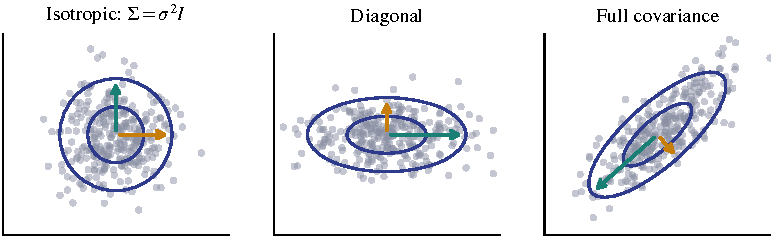
\includegraphics[width=0.86\linewidth]{figures/gaussian_2d.pdf}
\caption{Samples (grey) and the one- and two-$\sigma$ contour ellipses of three Gaussians in $d = 2$. Arrows are the
eigenvectors scaled by $2\sqrt{\lambda_i}$. The isotropic case has no preferred direction; the full covariance
captures a correlation between the two coordinates.}
\label{fig:gauss2d}
\end{figure}

\paragraph{Geometry through the eigendecomposition} Write $\Sigma = \sum_{i=1}^d \lambda_i \vect{v}_i \vect{v}_i\T$
with orthonormal eigenvectors $\vect{v}_i$ and eigenvalues $\lambda_i > 0$. The inverse has the same eigenvectors
and inverted eigenvalues, $\Sigma^{-1} = \sum_i \lambda_i^{-1} \vect{v}_i \vect{v}_i\T$ (multiply the two sums and use
$\vect{v}_i\T\vect{v}_j = 0$ for $i \ne j$, $=1$ for $i = j$). In matrix form $\Sigma = V\Lambda V\T$, where $V$ has
the $\vect{v}_i$ as columns and $\Lambda = \operatorname{diag}(\lambda_1, \dots, \lambda_d)$; we also write
$\Lambda^{1/2} = \operatorname{diag}(\sqrt{\lambda_1}, \dots, \sqrt{\lambda_d})$. In the rotated coordinates $u_i = \vect{v}_i\T(\x - \vmu)$
the exponent therefore becomes
\[
  (\x - \vmu)\T\Sigma^{-1}(\x - \vmu) = \sum_{i=1}^d \frac{\big(\vect{v}_i\T(\x - \vmu)\big)^2}{\lambda_i}
  = \sum_{i=1}^d \frac{u_i^2}{\lambda_i},
\]
so the density factorises into $d$ independent one-dimensional Gaussians with variances $\lambda_i$. This also
explains the prefactor of \eqref{eq:gaussnd}: the rotation $\vect{u} = V\T(\x - \vmu)$ preserves volumes (its
Jacobian is $1$), so
\[
  \int_{\R^d} e^{-\Delta^2(\x)/2}\,d\x = \prod_{i=1}^d \int_{-\infty}^{\infty} e^{-u_i^2/(2\lambda_i)}\,du_i
  = \prod_{i=1}^d \sqrt{2\pi\lambda_i} = (2\pi)^{d/2}\lvert\Sigma\rvert^{1/2} .
\]
The ellipsoid
$\Delta = 1$ has its axes along the eigenvectors with half-lengths $\sqrt{\lambda_i}$, and $\lvert\Sigma\rvert =
\prod_i \lambda_i$ is proportional to its squared volume (the volume is $V_d\sqrt{\lvert\Sigma\rvert}$, with $V_d$
the volume of the unit ball; $\pi\sqrt{\lvert\Sigma\rvert}$ in $d = 2$). Three families are common (Figure~\ref{fig:gauss2d}):

\begin{center}\small
\begin{tabular}{@{}L{0.18\linewidth}L{0.24\linewidth}L{0.22\linewidth}L{0.26\linewidth}@{}}
\toprule
Family & Covariance & Free parameters in $\Sigma$ & Shape \\
\midrule
Isotropic & $\sigma^2 I$ & $1$ & spheres \\
Diagonal & $\operatorname{diag}(\sigma_1^2, \dots, \sigma_d^2)$ & $d$ & axis-aligned ellipsoids \\
Full & any positive-definite $\Sigma$ & $d(d+1)/2$ & arbitrary ellipsoids \\
\bottomrule
\end{tabular}
\end{center}

The choice is a choice of model size. For $d = 1000$ a full covariance has about half a million parameters, which
$n = 500$ examples cannot determine; Note~4, Section~5, calls this a question of \emph{capacity}.

\subsection{A two-dimensional example with numbers}\label{sec:example2d}

One covariance matrix is worked through in full here; the same numbers return for conditioning
(Section~\ref{sec:conditioning}), sampling (Section~\ref{sec:sampling}) and log-densities
(Section~\ref{sec:logpdf}), so that every formula can be checked by hand.

\begin{worked}{eigenvalues, ellipse axes and Mahalanobis distance}
Take
\[
  \vmu = \begin{pmatrix} 1 \\ 2 \end{pmatrix}, \qquad
  \Sigma = \begin{pmatrix} 5 & 2 \\ 2 & 2 \end{pmatrix}.
\]
The variances are $5$ and $2$ and the correlation is $\rho = 2/\sqrt{5 \cdot 2} \approx 0.63$.

\emph{Eigenvalues.} They solve $\det(\Sigma - \lambda I) = (5 - \lambda)(2 - \lambda) - 4 = \lambda^2 - 7\lambda + 6
= 0$, so $\lambda_1 = 6$ and $\lambda_2 = 1$. Check: $\lambda_1 + \lambda_2 = 7 = \operatorname{tr}\Sigma$ and
$\lambda_1\lambda_2 = 6 = \lvert\Sigma\rvert$.

\emph{Eigenvectors.} For $\lambda_1 = 6$, the first row of $(\Sigma - 6I)\vect{v} = 0$ reads $-v_1 + 2v_2 = 0$, so
$\vect{v}_1 = (2, 1)/\sqrt5$. For $\lambda_2 = 1$, $4v_1 + 2v_2 = 0$ gives $\vect{v}_2 = (1, -2)/\sqrt5$. They are
orthogonal, as they must be for a symmetric matrix.

\emph{Ellipse.} The contour $\Delta = 1$ is an ellipse centred at $(1, 2)$ with long half-axis $\sqrt6 \approx 2.45$
along $(2, 1)$ --- tilted by $\arctan(1/2) \approx 26.6^\circ$ --- and short half-axis $\sqrt1 = 1$ along $(1, -2)$.
The contour $\Delta = 2$ is the same ellipse scaled by two (Figure~\ref{fig:example2d}, left). The area inside
$\Delta = 1$ is $\pi\sqrt{\lambda_1\lambda_2} = \pi\sqrt{\lvert\Sigma\rvert} = \pi\sqrt6 \approx 7.70$.

\emph{Mahalanobis distance.} The inverse is $\Sigma^{-1} = \frac16\begin{pmatrix} 2 & -2 \\ -2 & 5\end{pmatrix}$,
so for a displacement $\vect{r} = \x - \vmu$ the quadratic form is $\Delta^2 = \vect{r}\T\Sigma^{-1}\vect{r} =
(2r_1^2 - 4r_1r_2 + 5r_2^2)/6$ (the cross term appears twice). Compare two points at the \emph{same} Euclidean
distance $\sqrt5 \approx 2.24$ from the mean:
\begin{align*}
  A = (3, 3):&\quad \vect{r} = (2, 1), & \Delta^2 &= \tfrac16\,(2 \cdot 4 - 4 \cdot 2 \cdot 1 + 5 \cdot 1)
  = \tfrac56, & \Delta_A &\approx 0.91, \\
  B = (2, 0):&\quad \vect{r} = (1, -2), & \Delta^2 &= \tfrac16\,\big(2 \cdot 1 - 4 \cdot 1 \cdot (-2) + 5 \cdot 4\big)
  = 5, & \Delta_B &\approx 2.24 .
\end{align*}
The eigenvector form gives the same numbers: $\vect{r}_A = (2, 1) = \sqrt5\,\vect{v}_1$, so $\Delta^2 = 5/\lambda_1 =
5/6$, while $\vect{r}_B = (1, -2) = \sqrt5\,\vect{v}_2$, so $\Delta^2 = 5/\lambda_2 = 5$.
Point $A$ lies along the long axis, where the distribution is wide, and is unremarkable; $B$ lies along the short
axis and is more than two ``standard deviations'' out. The densities differ by a factor $e^{-(5 - 5/6)/2} \approx
0.12$: $\Normal(A) = e^{-5/12}/(2\pi\sqrt6) \approx 0.0428$ and $\Normal(B) = e^{-5/2}/(2\pi\sqrt6) \approx 0.0053$.
\end{worked}

\begin{figure}[tbp]
\centering
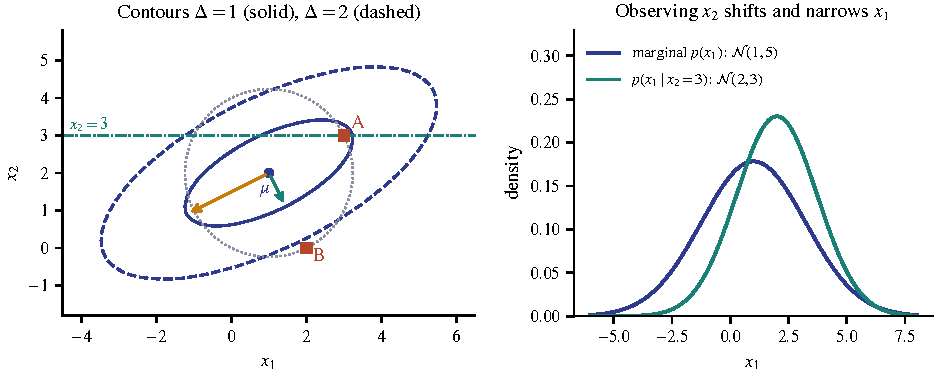
\includegraphics[width=0.86\linewidth]{figures/n2_example2d.pdf}
\caption{The worked examples of Sections~\ref{sec:example2d}--\ref{sec:conditioning}. Left: contours of
$\Normal(\vmu, \Sigma)$ with $\vmu = (1, 2)$, $\Sigma = \bigl(\begin{smallmatrix} 5 & 2 \\ 2 & 2\end{smallmatrix}\bigr)$; arrows are the eigenvectors scaled by
$\sqrt{\lambda_i}$; the dotted circle has Euclidean radius $\sqrt5$ and passes through both $A$ and $B$. Right: the
marginal of $x_1$ and its conditional on the line $x_2 = 3$.}
\label{fig:example2d}
\end{figure}

\subsection{How much probability lies inside an ellipse}\label{sec:coverage}

In one dimension, $68\%$ of the probability lies within $\Delta = \lvert x - \mu\rvert/\sigma \le 1$. This rule does
not carry over to higher dimension. In the rotated and rescaled coordinates $w_i = u_i/\sqrt{\lambda_i}$ the $w_i$
are independent standard normals and $\Delta^2 = \sum_i w_i^2$, a sum of $d$ squared standard normals: a
$\chi^2$ variable with $d$ degrees of freedom. In $d = 2$ the probability can be computed in polar coordinates
$(r, \varphi)$ for $(w_1, w_2)$. The joint density of $(w_1, w_2)$ is $\frac{1}{2\pi}e^{-(w_1^2 + w_2^2)/2}$, the
region $\Delta \le k$ is the disc $w_1^2 + w_2^2 \le k^2$, and $dw_1\,dw_2 = r\,dr\,d\varphi$, so
\[
  P(\Delta \le k) = \int_0^{2\pi}\!\!\int_0^k \frac{1}{2\pi} e^{-r^2/2}\, r\, dr\, d\varphi
  = \frac{2\pi}{2\pi}\int_0^k r\,e^{-r^2/2}\,dr
  = \Big[-e^{-r^2/2}\Big]_0^k = 1 - e^{-k^2/2} .
\]
The ellipses $\Delta = 1, 2, 3$ therefore contain $39.3\%$, $86.5\%$ and $98.9\%$ of the probability --- less than
in one dimension --- and the 95\% ellipse is $\Delta = \sqrt{-2\log 0.05} \approx 2.45$. As $d$ grows, the mass moves
further out: $\E[\Delta^2] = d$, and the typical sample lies at $\Delta \approx \sqrt d$ (Question~C4; Note~3,
Section~3).

\subsection{Marginals and conditionals}\label{sec:conditioning}

\paragraph{Closed under marginalising and conditioning} Split $\x = (\x_a, \x_b)$ into $d_a$ coordinates to be
predicted and $d_b$ observed ones, and partition the mean and covariance in the same way,
\[
  \vmu = \begin{pmatrix} \vmu_a \\ \vmu_b \end{pmatrix}, \qquad
  \Sigma = \begin{pmatrix} \Sigma_{aa} & \Sigma_{ab} \\ \Sigma_{ba} & \Sigma_{bb} \end{pmatrix}, \qquad
  \Sigma_{ba} = \Sigma_{ab}\T ,
\]
where $\Sigma_{ab} = \Cov(\x_a, \x_b)$ is $d_a \times d_b$. In the example of Section~\ref{sec:example2d} with
$a = \{1\}$ and $b = \{2\}$, $\Sigma_{aa} = 5$, $\Sigma_{ab} = \Sigma_{ba} = 2$ and $\Sigma_{bb} = 2$. Every marginal of a Gaussian is Gaussian --- just keep the corresponding entries,
$\x_a \sim \Normal(\vmu_a, \Sigma_{aa})$ --- and every conditional is Gaussian,
\begin{equation}\label{eq:conditional}
  \x_a \mid \x_b \sim \Normal\!\big( \vmu_a + \Sigma_{ab}\Sigma_{bb}^{-1}(\x_b - \vmu_b),\;
  \Sigma_{aa} - \Sigma_{ab}\Sigma_{bb}^{-1}\Sigma_{ba} \big).
\end{equation}
The conditional mean is linear in the observed part and the conditional covariance does not depend on it. Since a
Gaussian density peaks at its mean, the conditional mean is also the single most probable value of $\x_a$, so both
readings of ``infer'' in Section~\ref{sec:operations} give the same answer. This is
inference in closed form: if two detector channels are correlated, reading one sharpens the prediction for the
other by an amount set by the correlation. Formula \eqref{eq:conditional} underlies the Kalman filter used for
particle-track reconstruction and spacecraft navigation, and Gaussian-process regression.

\paragraph{Where the formula comes from (two dimensions)} Let $(X_1, X_2)$ be jointly Gaussian with variances
$\Sigma_{11}, \Sigma_{22}$ and covariance $\Sigma_{12}$. Split $X_1$ into a part explained by $X_2$ and a remainder,
\[
  X_1 = \mu_1 + \beta\,(X_2 - \mu_2) + E, \qquad \beta = \frac{\Sigma_{12}}{\Sigma_{22}} .
\]
This only \emph{defines} $E = X_1 - \beta X_2 + \text{const}$. Its mean is zero, and because covariance is linear
in each argument (and ignores constants), its covariance with $X_2$ is
\[
  \Cov(E, X_2) = \Cov(X_1, X_2) - \beta\Var(X_2) = \Sigma_{12} - \frac{\Sigma_{12}}{\Sigma_{22}}\Sigma_{22} = 0 .
\]
$E$ is a linear function of the Gaussian vector $(X_1, X_2)$, so $(E, X_2)$ is jointly Gaussian by \eqref{eq:gausslin}, and for jointly Gaussian variables
zero covariance implies independence (the density factorises because $\Sigma$ is then diagonal). Knowing $X_2 = x_2$
thus leaves the distribution of $E$ unchanged, and
\begin{align*}
  \E[X_1 \mid X_2 = x_2] &= \mu_1 + \frac{\Sigma_{12}}{\Sigma_{22}}(x_2 - \mu_2), \\
  \Var(X_1 \mid X_2 = x_2) &= \Var(E) = \Var(X_1) - 2\beta\Cov(X_1, X_2) + \beta^2\Var(X_2)
  = \Sigma_{11} - \frac{\Sigma_{12}^2}{\Sigma_{22}} ,
\end{align*}
which is \eqref{eq:conditional} for $d = 2$. The variance of $E = X_1 - \beta X_2 + \text{const}$ is
\eqref{eq:covlin} with the row $A = (1, -\beta)$: $(1, -\beta)\,\Sigma\,(1, -\beta)\T = \Sigma_{11} - 2\beta\Sigma_{12}
+ \beta^2\Sigma_{22}$, and inserting $\beta = \Sigma_{12}/\Sigma_{22}$ gives the last expression. In terms of the correlation, the conditional variance is
$\Sigma_{11}(1 - \rho^2)$: observing $X_2$ removes the fraction $\rho^2$ of the variance of $X_1$. The same argument
with matrices, $B = \Sigma_{ab}\Sigma_{bb}^{-1}$ in place of $\beta$, gives the general case (Question~C5).

\begin{worked}{conditioning the two-dimensional example}
For $\vmu = (1, 2)$ and $\Sigma = \bigl(\begin{smallmatrix} 5 & 2 \\ 2 & 2\end{smallmatrix}\bigr)$, suppose we observe $X_2 = 3$. Then
\[
  \E[X_1 \mid X_2 = 3] = 1 + \frac{2}{2}\,(3 - 2) = 2, \qquad
  \Var(X_1 \mid X_2 = 3) = 5 - \frac{2^2}{2} = 3 .
\]
Before the observation $X_1 \sim \Normal(1, 5)$; after it $X_1 \sim \Normal(2, 3)$ (Figure~\ref{fig:example2d}, right).
The observed $x_2$ lies one unit above its mean; with the slope $\beta = \Sigma_{12}/\Sigma_{22} = 1$ this pulls the
prediction of $x_1$ up by one unit, and the variance shrinks by the fraction $\rho^2 = 4/10 = 0.4$. The roles can be reversed: given $X_1 = 3$,
$X_2 \sim \Normal(2 + \frac25 \cdot 2, \; 2 - \frac45) = \Normal(2.8, 1.2)$.
\end{worked}

In computation, $\Sigma_{bb}^{-1}$ is never formed: with the Cholesky factor of Section~\ref{sec:sampling},
$\Sigma_{bb} = L_bL_b\T$, both products in \eqref{eq:conditional} reduce to triangular solves, since
$\Sigma_{ab}\Sigma_{bb}^{-1}\Sigma_{ba} = W\T W$ with $W = L_b^{-1}\Sigma_{ba}$ (Algorithm~\ref{alg:condition}). For
the example above, $L_b = \sqrt2$, $W = 2/\sqrt2 = \sqrt2$ and $\vect{u} = (3 - 2)/\sqrt2$, so the mean is $1 + W u = 2$
and the variance $5 - W^2 = 3$, as before.

\begin{algorithm}[htbp]
\caption{Conditioning a Gaussian on observed coordinates $\x_b$}\label{alg:condition}
\begin{algorithmic}[1]
\Require blocks $\vmu_a, \vmu_b, \Sigma_{aa}, \Sigma_{ab}, \Sigma_{bb}$ ($d_a$ predicted and $d_b$ observed coordinates); observed $\x_b$
\Ensure mean and covariance of $\x_a \mid \x_b$, equation \eqref{eq:conditional}
\Function{Condition}{$\vmu, \Sigma, \x_b$}
  \State $L_b \gets$ \Call{Cholesky}{$\Sigma_{bb}$} \Comment{Algorithm~\ref{alg:gausssample}}
  \State solve $L_b W = \Sigma_{ba}$ for $W \in \R^{d_b \times d_a}$ \Comment{forward substitution, one column at a time}
  \State solve $L_b \vect{u} = \x_b - \vmu_b$ for $\vect{u} \in \R^{d_b}$
  \State \Return $\vmu_a + W\T\vect{u}$, \ $\Sigma_{aa} - W\T W$
\EndFunction
\end{algorithmic}
\end{algorithm}

\begin{runtime}{conditioning a Gaussian}
\emph{Set-up}: $O(d_b^3)$ for the Cholesky factor of $\Sigma_{bb}$, $O(d_a d_b^2)$ for the $d_a$ triangular solves that
give $W$, and $O(d_a^2 d_b)$ for the product $W\T W$; memory $O(d_b^2 + d_a d_b + d_a^2)$. \emph{Per new observation}
$\x_b$: $O(d_b^2)$ for one solve plus $O(d_a d_b)$ for $W\T\vect{u}$, or only $O(d_a d_b)$ if the matrix
$B = \Sigma_{ab}\Sigma_{bb}^{-1}$ is stored. The $O(d_b^3)$ term is why exact Gaussian-process regression, which
conditions on $n$ observed training targets, costs $O(n^3)$.
\end{runtime}

\section{Sampling: from white noise to anything Gaussian}\label{sec:sampling}

To sample $\Normal(\vmu, \Sigma)$, factor $\Sigma = LL\T$ (Cholesky decomposition, $L$ lower triangular with positive
diagonal), draw $\vect{z} \sim \Normal(\vect{0}, I)$ --- $d$ independent standard normals --- and return
\begin{equation}\label{eq:reparam}
  \x = \vmu + L \vect{z}.
\end{equation}
\paragraph{Why this has covariance $\Sigma$} The vector $\vect{z}$ has mean $\vect{0}$ and covariance $I$, because its
components are independent with unit variance. Apply the rules of Section~\ref{sec:moments} with $A = L$ and
$\vect{b} = \vmu$:
\[
  \E[\x] = L\,\E[\vect{z}] + \vmu = \vmu, \qquad
  \Cov(\x) = L\,\Cov(\vect{z})\,L\T = L\,I\,L\T = LL\T = \Sigma .
\]
A linear map of a Gaussian vector is again Gaussian \eqref{eq:gausslin}, and a Gaussian is fixed by its mean and covariance, so
$\x \sim \Normal(\vmu, \Sigma)$. Any $L$ with $LL\T = \Sigma$ would do --- for instance $L = V\Lambda^{1/2}$ from the
eigendecomposition $\Sigma = V\Lambda V\T$ of Section~\ref{sec:gaussnd}, which samples independently along each ellipse axis --- but $\x = \vmu +
\Sigma\vect{z}$ would not: its covariance is $\Sigma\Sigma\T = \Sigma^2$.

\paragraph{The Cholesky factor by hand} For a $2 \times 2$ matrix, multiply out $LL\T$ and match entries:
\[
  \begin{pmatrix} L_{11} & 0 \\ L_{21} & L_{22} \end{pmatrix}
  \begin{pmatrix} L_{11} & L_{21} \\ 0 & L_{22} \end{pmatrix}
  = \begin{pmatrix} L_{11}^2 & L_{11}L_{21} \\ L_{11}L_{21} & L_{21}^2 + L_{22}^2 \end{pmatrix}
  \quad\Longrightarrow\quad
  L_{11} = \sqrt{\Sigma_{11}}, \ \ L_{21} = \frac{\Sigma_{21}}{L_{11}}, \ \
  L_{22} = \sqrt{\Sigma_{22} - L_{21}^2} .
\]
Read column by column, the same matching gives the general algorithm below. The square roots exist exactly when
$\Sigma$ is positive definite, so a failing Cholesky factorisation is the standard numerical test that a matrix is
not a valid covariance.

The standard normals themselves are produced by libraries from uniform random numbers, for example by the
Box--Muller transform~\cite{boxmuller1958}, the polar-coordinate computation of Section~\ref{sec:coverage} run
backwards: for independent uniforms $u_1 \in (0, 1]$ and $u_2 \in [0, 1)$, the numbers $z_1 = \sqrt{-2\log u_1}\cos(2\pi
u_2)$ and $z_2 = \sqrt{-2\log u_1}\sin(2\pi u_2)$ are two independent standard normals, at $O(1)$ cost per pair.

\begin{worked}{drawing one sample by hand}
For $\vmu = (1, 2)$ and $\Sigma = \bigl(\begin{smallmatrix} 5 & 2 \\ 2 & 2\end{smallmatrix}\bigr)$ of Section~\ref{sec:example2d}: $L_{11} = \sqrt5 \approx
2.2361$, $L_{21} = 2/\sqrt5 \approx 0.8944$, $L_{22} = \sqrt{2 - 4/5} = \sqrt{1.2} \approx 1.0954$. Check:
$L_{21}^2 + L_{22}^2 = 0.8 + 1.2 = 2$. With the standard-normal draw $\vect{z} = (1, -0.5)$,
\[
  \x = \begin{pmatrix} 1 \\ 2 \end{pmatrix} + \begin{pmatrix} 2.2361 & 0 \\ 0.8944 & 1.0954 \end{pmatrix}
  \begin{pmatrix} 1 \\ -0.5 \end{pmatrix}
  = \begin{pmatrix} 1 + 2.2361 \\ 2 + 0.8944 - 0.5477 \end{pmatrix} = \begin{pmatrix} 3.2361 \\ 2.3467 \end{pmatrix}.
\]
The first coordinate uses only $z_1$; the second mixes in $z_1$ through $L_{21}$, which is how the correlation
enters.
\end{worked}

\begin{algorithm}[htbp]
\caption{Cholesky factorisation and sampling from $\Normal(\vmu, \Sigma)$}\label{alg:gausssample}
\begin{algorithmic}[1]
\Require symmetric positive-definite $\Sigma \in \R^{d \times d}$, mean $\vmu \in \R^d$, number of samples $s$
\Ensure lower-triangular $L$ with $LL\T = \Sigma$; samples $\x_1, \dots, \x_s$
\Function{Cholesky}{$\Sigma$}
  \For{$j = 1, \dots, d$}
    \State $a \gets \Sigma_{jj} - \sum_{k<j} L_{jk}^2$
    \If{$a \le 0$} \textbf{stop}: $\Sigma$ is not positive definite \EndIf
    \State $L_{jj} \gets \sqrt{a}$
    \For{$i = j+1, \dots, d$}
      \State $L_{ij} \gets \big(\Sigma_{ij} - \sum_{k<j} L_{ik}L_{jk}\big) / L_{jj}$
    \EndFor
  \EndFor
  \State \Return $L$ \Comment{entries above the diagonal are zero}
\EndFunction
\Function{SampleGaussian}{$\vmu, \Sigma, s$}
  \State $L \gets$ \Call{Cholesky}{$\Sigma$} \Comment{once, reused for every sample}
  \For{$t = 1, \dots, s$}
    \State draw $\vect{z} \in \R^d$ with independent $\Normal(0, 1)$ entries
    \State $\x_t \gets \vmu + L\vect{z}$ \Comment{equation \eqref{eq:reparam}}
  \EndFor
  \State \Return $\x_1, \dots, \x_s$
\EndFunction
\end{algorithmic}
\end{algorithm}

\keeplines{8}
\begin{runtime}{sampling a multivariate Gaussian}
\emph{Factorisation}: Cholesky costs about $d^3/3$ floating-point operations ($d^3/6$ multiply--adds), $O(d^3)$ ---
the double loop over $(i, j)$ with an inner sum of length $j$ --- and is done once; memory $O(d^2)$ for $L$.
\emph{Per sample}: $O(d)$ for the normals plus $O(d^2)$ for the triangular product $L\vect{z}$.
\emph{Total} for $s$ samples: $O(d^3 + s\,d^2)$; stacking the $\vect{z}$'s as columns of a $d \times s$ matrix turns the
loop into one matrix product. For $d = 10^3$ the factorisation takes about $3 \times 10^8$ operations; for $d \sim
10^5$ a full $\Sigma$ ($10^{10}$ entries, $80$~GB in double precision) exceeds a workstation or a GPU and its
factorisation costs about $3 \times 10^{14}$ operations, which is why the isotropic case $\x = \vmu + \sigma\vect{z}$, at
$O(d)$ per sample, dominates in high dimension.
\end{runtime}

\begin{modern}{Gaussian noise drives generative models}
Equation \eqref{eq:reparam} separates the randomness ($\vect{z}$) from the parameters ($\vmu, L$). Variational
autoencoders exploit this ``reparameterisation trick'' to differentiate through sampling~\cite{kingma2014}.
Diffusion models, behind many of today's image generators, go further. Their \emph{forward process}
gradually turns data into noise: with $\bar\alpha_t$ decreasing from $1$ to nearly $0$,
\[
  \x_t = \sqrt{\bar\alpha_t}\, \x_0 + \sqrt{1 - \bar\alpha_t}\, \vect{z}, \qquad \vect{z} \sim \Normal(\vect{0}, I),
\]
so $\x_t \mid \x_0 \sim \Normal(\sqrt{\bar\alpha_t}\,\x_0, (1 - \bar\alpha_t) I)$, an isotropic Gaussian
(Figure~\ref{fig:diffusion}). The two coefficients are chosen so that the variance is preserved. Because $\vect{z}$
is drawn independently of $\x_0$, the variances of the two terms add: if each component of $\x_0$ has unit variance,
then $\Var(x_{t,j}) = \bar\alpha_t \cdot 1 + (1 - \bar\alpha_t) \cdot 1 = 1$ for every component $j$ at every step. A neural network is trained to
predict $\vect{z}$ from $\x_t$ and $t$; running the process backwards from pure noise then generates new
samples~\cite{ho2020,song2021}. Everything in this section --- isotropic covariances, scaling and shifting, sampling
by \eqref{eq:reparam} --- is used literally.
\end{modern}

\begin{figure}[htbp]
\centering
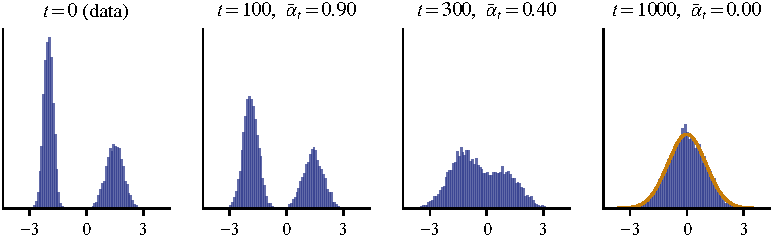
\includegraphics[width=0.9\linewidth]{figures/diffusion_forward.pdf}
\caption{The forward process of a diffusion model applied to a one-dimensional, two-peaked data distribution
(histograms of $10^4$ samples, the noise schedule of Ho \emph{et al.}~\cite{ho2020} with $1000$ steps). By the
last step the data are indistinguishable from $\Normal(0, 1)$ (curve).}
\label{fig:diffusion}
\end{figure}

\section{Learning the parameters}\label{sec:learn}

Given $\x_1, \dots, \x_n \in \R^d$, the maximum-likelihood estimates of a Gaussian are the empirical mean and
covariance,
\begin{equation}\label{eq:mlegauss}
  \hat{\vmu} = \frac{1}{n}\sum_{i=1}^n \x_i, \qquad
  \hat\Sigma = \frac{1}{n}\sum_{i=1}^n (\x_i - \hat{\vmu})(\x_i - \hat{\vmu})\T = \frac{1}{n} X_c\T X_c ,
\end{equation}
where $X_c$ is the design matrix of Note~1 with $\hat{\vmu}$ subtracted from every row. Entry by entry,
$\hat\Sigma_{jk} = \frac1n\sum_i (x_{i,j} - \hat\mu_j)(x_{i,k} - \hat\mu_k)$.

\subsection{Maximum likelihood in one dimension}\label{sec:mle1d}

Write $v = \sigma^2$ to avoid confusing derivatives with respect to $\sigma$ and $\sigma^2$. Taking the logarithm of
\eqref{eq:gauss1d} for each point and adding,
\[
  \ell(\mu, v) = \sum_{i=1}^n \log\Normal(x_i; \mu, v) = -\frac{n}{2}\log(2\pi) - \frac{n}{2}\log v
  - \frac{1}{2v}\sum_{i=1}^n (x_i - \mu)^2 .
\]
\emph{Mean.} Only the last term depends on $\mu$. Using $\frac{d}{d\mu}(x_i - \mu)^2 = -2(x_i - \mu)$,
\[
  \frac{\partial\ell}{\partial\mu} = \frac{1}{v}\sum_{i=1}^n (x_i - \mu) = \frac{1}{v}\Big(\sum_i x_i - n\mu\Big) = 0
  \quad\Longrightarrow\quad \hat\mu = \frac1n\sum_{i=1}^n x_i = \bar x .
\]
\emph{Variance.} With $\frac{d}{dv}\log v = 1/v$ and $\frac{d}{dv}(1/v) = -1/v^2$,
\[
  \frac{\partial\ell}{\partial v} = -\frac{n}{2v} + \frac{1}{2v^2}\sum_{i=1}^n (x_i - \mu)^2 = 0
  \quad\Longrightarrow\quad \hat v = \hat\sigma^2 = \frac1n\sum_{i=1}^n (x_i - \bar x)^2 ,
\]
after multiplying by $2v^2/n$ and inserting $\mu = \hat\mu$. Both stationary points are maxima: $\ell$ is a downward
parabola in $\mu$, and in $v$ it tends to $-\infty$ both as $v \to 0$ and as $v \to \infty$, with a single stationary
point in between.

\begin{worked}{fitting a one-dimensional Gaussian}
Five repeated measurements give $4, 7, 5, 9, 5$. The mean is $\bar x = 30/5 = 6$. The deviations are $-2, 1, -1, 3,
-1$ (they sum to zero, a useful check), their squares $4, 1, 1, 9, 1$ sum to $16$, so $\hat\sigma^2 = 16/5 = 3.2$ and
$\hat\sigma \approx 1.79$. The unbiased version of the next subsection divides by $n - 1 = 4$ and gives $4.0$.
\end{worked}

\subsection{The \texorpdfstring{$1/n$}{1/n} variance is biased}\label{sec:bias}

An estimator is \emph{unbiased} if its average over many datasets equals the true value. Let $x_1, \dots, x_n$ be
i.i.d.\ with mean $\mu$ and variance $\sigma^2$; in this subsection the $x_i$ and $\bar x$ denote random variables
(the data of a dataset not yet drawn). First expand the sum of squared deviations:
\[
  \sum_i (x_i - \bar x)^2 = \sum_i x_i^2 - 2\bar x\sum_i x_i + n\bar x^2 = \sum_i x_i^2 - n\bar x^2 ,
\]
using $\sum_i x_i = n\bar x$. Next, $\Var(X) = \E[X^2] - (\E[X])^2$ (Section~\ref{sec:moments}) gives
$\E[x_i^2] = \Var(x_i) + \mu^2 = \sigma^2 + \mu^2$. For $\bar x$, the vector $(x_1, \dots, x_n)$ has covariance
$\sigma^2 I$ because the $x_i$ are independent, and \eqref{eq:covlin} with the row $A = (\frac1n, \dots, \frac1n)$
gives $\Var(\bar x) = \sigma^2 \cdot n/n^2 = \sigma^2/n$, so $\E[\bar x^2] = \sigma^2/n + \mu^2$. Therefore
\[
  \E\Big[\sum_i (x_i - \bar x)^2\Big] = n(\sigma^2 + \mu^2) - n\Big(\frac{\sigma^2}{n} + \mu^2\Big) = (n - 1)\,\sigma^2 ,
\]
and $\E[\hat\sigma^2] = \frac{n-1}{n}\sigma^2$. The deviations are measured from $\bar x$, which was fitted to the same
points and is therefore closer to them than the true $\mu$; one ``degree of freedom'' is used up by the mean. This
is why statistics software often divides by $n - 1$. The same holds for every entry of $\hat\Sigma$. For the sample
sizes of machine learning the difference is negligible (a relative change of $10^{-6}$ for $n = 10^6$), but for
$n = 5$ it is 20\%.

\subsection{The multivariate case}\label{sec:mlend}

Before deriving \eqref{eq:mlegauss} in $d$ dimensions, here it is at work on a small dataset.

\begin{worked}{fitting a mean and a covariance to five points}
Fit a two-dimensional Gaussian to $(1, 2)$, $(2, 3)$, $(3, 3)$, $(4, 5)$, $(5, 7)$.
\begin{itemize}
\item \emph{Mean:} $\hat{\vmu} = \big(\frac{1+2+3+4+5}{5}, \frac{2+3+3+5+7}{5}\big) = (3, 4)$.
\item \emph{Centred points} (rows of $X_c$): $(-2, -2)$, $(-1, -1)$, $(0, -1)$, $(1, 1)$, $(2, 3)$; each column sums
to zero.
\item \emph{Sums of products:} $\sum c_1^2 = 4 + 1 + 0 + 1 + 4 = 10$; \ $\sum c_2^2 = 4 + 1 + 1 + 1 + 9 = 16$; \
$\sum c_1c_2 = 4 + 1 + 0 + 1 + 6 = 12$.
\item \emph{Covariance:} dividing by $n = 5$,
$\hat\Sigma = \begin{pmatrix} 2 & 2.4 \\ 2.4 & 3.2 \end{pmatrix}$; dividing by $n - 1 = 4$ instead gives
$\begin{pmatrix} 2.5 & 3 \\ 3 & 4 \end{pmatrix}$.
\end{itemize}
The fitted correlation is $2.4/\sqrt{2 \times 3.2} \approx 0.95$: the points lie close to a rising line. The
eigenvalues of $\hat\Sigma$ are about $5.07$ and $0.13$, so the fitted ellipse is long and thin, and $\lvert\hat\Sigma\rvert
= 2 \times 3.2 - 2.4^2 = 0.64$.
\end{worked}

The log-likelihood of $n$ points under \eqref{eq:gaussnd} is
\[
  \ell(\vmu, \Sigma) = -\frac{nd}{2}\log(2\pi) - \frac{n}{2}\log\lvert\Sigma\rvert
  - \frac12\sum_{i=1}^n (\x_i - \vmu)\T\Sigma^{-1}(\x_i - \vmu) .
\]
We sketch the two steps; Bishop~\cite{bishop2006}, Section~2.3.4, derives the mean and states the covariance
result, whose derivation is his Exercise~2.34.

\emph{Mean.} For a symmetric matrix $A$, the gradient of the quadratic form $(\x - \vmu)\T A(\x - \vmu)$ with respect
to $\vmu$ is $-2A(\x - \vmu)$, the vector version of $\frac{d}{d\mu}a(x - \mu)^2 = -2a(x - \mu)$ (Note~7, Section~2).
Setting the gradient of $\ell$ to zero, $\Sigma^{-1}\sum_i (\x_i - \vmu) = \vect{0}$, and multiplying by $\Sigma$ gives
$\hat{\vmu} = \frac1n\sum_i \x_i$. The covariance plays no role, exactly as in one dimension.

\emph{Covariance (optional, for the interested reader).} The quickest check is a diagonal $\Sigma$: then $\ell$
splits into $d$ one-dimensional log-likelihoods, one per coordinate, and Section~\ref{sec:mle1d} gives
$\hat\Sigma_{jj} = \frac1n\sum_i (x_{i,j} - \hat\mu_j)^2$, the diagonal of \eqref{eq:mlegauss}. For a full $\Sigma$ it
is easiest to differentiate with respect to the \emph{precision matrix} $Q = \Sigma^{-1}$, using matrix calculus beyond
this course. Since $\log\lvert\Sigma\rvert = -\log\lvert Q\rvert$ and a number equals its own trace, $\vect{a}\T Q\vect{a} =
\operatorname{tr}(Q\vect{a}\vect{a}\T)$, the log-likelihood at $\vmu = \hat{\vmu}$ becomes
\[
  \ell = \text{const} + \frac{n}{2}\log\lvert Q\rvert - \frac12\operatorname{tr}(Q S), \qquad
  S = \sum_{i=1}^n (\x_i - \hat{\vmu})(\x_i - \hat{\vmu})\T .
\]
Two standard matrix derivatives, $\partial\log\lvert Q\rvert/\partial Q = Q^{-1}$ and
$\partial\operatorname{tr}(QS)/\partial Q = S$ (treating the $d^2$ entries of $Q$ as independent; imposing the
symmetry of $Q$ changes both gradients in the same way and gives the same stationary point), give
\[
  \frac{\partial\ell}{\partial Q} = \frac n2 Q^{-1} - \frac12 S = 0 \quad\Longrightarrow\quad
  \hat\Sigma = Q^{-1} = \frac{S}{n},
\]
which is \eqref{eq:mlegauss}. For $d = 1$, $Q = 1/v$ and the two derivatives are $1/Q = v$ and $S$: the
computation is the one of Section~\ref{sec:mle1d}.

\subsection{When \texorpdfstring{$n$}{n} is not much larger than \texorpdfstring{$d$}{d}}\label{sec:shrinkage}

The matrix $\hat\Sigma = X_c\T X_c / n$ has rank at most $n - 1$ (the $n$ rows of $X_c$ sum to zero, so at most $n - 1$
of them are independent), so for $n \le d$ it is singular: the fitted Gaussian is flat in some directions and
\eqref{eq:gaussnd} cannot be evaluated. Even for $n$ somewhat larger than $d$ its small eigenvalues are badly
underestimated, and directions that happened to show little spread in the sample are treated as if almost nothing
could vary along them. The usual remedies are to restrict the family (diagonal or isotropic) or to \emph{shrink},
\[
  \hat\Sigma_\epsilon = \hat\Sigma + \epsilon I \qquad\text{or}\qquad
  \hat\Sigma_\gamma = (1 - \gamma)\,\hat\Sigma + \gamma\,\frac{\operatorname{tr}\hat\Sigma}{d}\,I, \quad 0 \le \gamma \le 1 .
\]
Adding $\epsilon I$ keeps the eigenvectors and raises every eigenvalue by $\epsilon$, so the matrix becomes
invertible; the second form pulls the eigenvalues towards their average, and Ledoit and Wolf~\cite{ledoit2004} showed
how to choose $\gamma$ from the data. Both are the simplest instance of the regularisation discussed in Note~4,
Section~7: a little bias in exchange for a large reduction in variance.

\begin{algorithm}[htbp]
\caption{Fitting a Gaussian by maximum likelihood, with optional shrinkage}\label{alg:gaussfit}
\begin{algorithmic}[1]
\Require data $\x_1, \dots, \x_n \in \R^d$ (rows of $X$); family $\in \{$full, diagonal, isotropic$\}$; $\epsilon \ge 0$
\Ensure $\hat{\vmu} \in \R^d$ and $\hat\Sigma \in \R^{d \times d}$
\Function{FitGaussian}{$X$, family, $\epsilon$}
  \State $\hat{\vmu} \gets \frac1n\sum_{i=1}^n \x_i$ \Comment{column means}
  \State $X_c \gets X - \vect{1}\hat{\vmu}\T$ \Comment{subtract the mean from every row}
  \If{family $=$ full}
    \State $\hat\Sigma \gets \frac1n X_c\T X_c$ \Comment{equation \eqref{eq:mlegauss}}
  \ElsIf{family $=$ diagonal}
    \State $\hat\Sigma \gets \operatorname{diag}(v_1, \dots, v_d)$ with $v_j = \frac1n\sum_i (X_c)_{ij}^2$
  \Else
    \State $\hat\Sigma \gets v\,I$ with $v = \frac{1}{nd}\sum_{i,j} (X_c)_{ij}^2$
  \EndIf
  \State $\hat\Sigma \gets \hat\Sigma + \epsilon I$ \Comment{shrinkage; $\epsilon = 0$ is plain maximum likelihood}
  \State \Return $\hat{\vmu}, \hat\Sigma$
\EndFunction
\end{algorithmic}
\end{algorithm}

\begin{runtime}{fitting a Gaussian}
\emph{Mean and centring}: $O(nd)$, one pass over the data. \emph{Full covariance}: $O(nd^2)$ for the product
$X_c\T X_c$ ($d^2$ entries, each a sum of $n$ terms; half of them suffice by symmetry). \emph{Diagonal or
isotropic}: $O(nd)$. \emph{Shrinkage}: $O(d)$. Memory: $O(d^2)$ for a full $\hat\Sigma$, $O(d)$ otherwise. For $n = 10^6$ and $d = 10^3$ the product $X_c\T X_c$
is $10^{12}$ multiply--adds, but a single matrix multiplication, which GPUs do best. There is no training loop: the
fit is in closed form, unlike most models of this course (Note~7).
\end{runtime}

\begin{worked}{two points in two dimensions}
From $(0, 0)$ and $(2, 2)$: $\hat{\vmu} = (1, 1)$ and $\hat\Sigma = \bigl(\begin{smallmatrix} 1 & 1 \\ 1 & 1\end{smallmatrix}\bigr)$,
with eigenvalues $2$ (along $(1,1)$) and $0$ (along $(1,-1)$) and determinant $0$. The fitted Gaussian lives on the
line $x_1 = x_2$ and assigns zero density to every point off it. With $\epsilon = 0.1$ the eigenvalues become $2.1$
and $0.1$, and $\lvert\hat\Sigma_\epsilon\rvert = 0.21$. Now every point has a finite Mahalanobis distance. With the
eigenvectors $\vect{v}_1 = (1, 1)/\sqrt2$, $\vect{v}_2 = (1, -1)/\sqrt2$ and $\Delta^2 = (\vect{r}\T\vect{v}_1)^2/2.1 +
(\vect{r}\T\vect{v}_2)^2/0.1$: the training point $(2, 2)$ has $\vect{r} = (1, 1)$, $\vect{r}\T\vect{v}_1 = \sqrt2$,
$\vect{r}\T\vect{v}_2 = 0$, so $\Delta^2 = 2/2.1 \approx 0.95$; the point $(1, 0)$, which lies off the line, has
$\vect{r} = (0, -1)$, $\vect{r}\T\vect{v}_1 = -1/\sqrt2$, $\vect{r}\T\vect{v}_2 = 1/\sqrt2$, so $\Delta^2 = 0.5/2.1 + 0.5/0.1
\approx 0.24 + 5 = 5.24$. The $1/\epsilon$ term dominates. The value of
$\epsilon$ sets how strongly ``off the line'' is penalised; it is chosen on validation data (Note~4).
\end{worked}

\subsection{Computing log-densities}\label{sec:logpdf}

In practice one evaluates $\log \Normal(\x; \vmu, \Sigma)$, never the density itself, which underflows in high
dimension: with $d = 1000$, $\lvert\Sigma\rvert = 1$ and $\Delta^2 \approx d$, the factor $e^{-\Delta^2/2} \approx
e^{-500} \approx 10^{-217}$ and the prefactor $(2\pi)^{-d/2} \approx 10^{-399}$ together give a density of order
$10^{-616}$, far below the smallest positive double-precision number (about $10^{-308}$, or $10^{-324}$ counting
subnormals), while its logarithm, about $-1419$, is an ordinary number. With $\Sigma = LL\T$, solve the triangular system $L\vect{u} = \x - \vmu$; then
\[
  \Delta^2 = (\x - \vmu)\T(LL\T)^{-1}(\x - \vmu) = (L^{-1}(\x - \vmu))\T(L^{-1}(\x - \vmu)) = \norm{\vect{u}}^2,
  \qquad \log\lvert\Sigma\rvert = \log\lvert L\rvert^2 = 2\sum_i \log L_{ii},
\]
because the determinant of a triangular matrix is the product of its diagonal. No matrix is ever inverted: a
triangular system is solved by \emph{forward substitution}, $u_1 = r_1/L_{11}$, then $u_2 = (r_2 - L_{21}u_1)/L_{22}$,
and so on, which is both faster and more accurate than forming $\Sigma^{-1}$. In numpy the two steps are
\texttt{np.linalg.cholesky} and \texttt{scipy.linalg.solve\_triangular}, the second applied to all rows of $X$ at
once (Algorithm~\ref{alg:logpdf}).

\begin{algorithm}[htbp]
\caption{Gaussian log-density of many points via Cholesky}\label{alg:logpdf}
\begin{algorithmic}[1]
\Require points $\x_1, \dots, \x_n \in \R^d$; mean $\vmu$; positive-definite $\Sigma$
\Ensure $g_i = \log\Normal(\x_i; \vmu, \Sigma)$ for $i = 1, \dots, n$
\Function{GaussLogPdf}{$X, \vmu, \Sigma$}
  \State $L \gets$ \Call{Cholesky}{$\Sigma$} \Comment{Algorithm~\ref{alg:gausssample}, once}
  \State $h \gets \sum_{j=1}^d \log L_{jj}$ \Comment{$h = \frac12\log\lvert\Sigma\rvert$}
  \For{$i = 1, \dots, n$}
    \State $\vect{r} \gets \x_i - \vmu$
    \For{$j = 1, \dots, d$} \Comment{forward substitution for $L\vect{u} = \vect{r}$}
      \State $u_j \gets \big(r_j - \sum_{k<j} L_{jk}u_k\big)/L_{jj}$
    \EndFor
    \State $g_i \gets -\frac12\norm{\vect{u}}^2 - h - \frac d2\log(2\pi)$
  \EndFor
  \State \Return $g_1, \dots, g_n$
\EndFunction
\end{algorithmic}
\end{algorithm}

\begin{runtime}{evaluating Gaussian log-densities}
\emph{Set-up}: Cholesky $O(d^3)$ and the log-determinant $O(d)$, once per Gaussian. \emph{Per query point}: $O(d^2)$
for the forward substitution (row $j$ needs $j$ products) plus $O(d)$ for the norm. \emph{Total}: $O(d^3 + nd^2)$
time and $O(d^2)$ memory, plus $O(nd)$ if all points are solved at once. Inverting $\Sigma$ explicitly costs the same order but loses accuracy
when $\Sigma$ is badly conditioned. With a diagonal $\Sigma$ everything is $O(d)$ per point. In a Gaussian Bayes
classifier (Note~6, Section~3) the set-up is repeated for each of the $m$ classes: $O(md^3 + nmd^2)$.
\end{runtime}

\begin{worked}{a log-density by Cholesky}
For the example of Section~\ref{sec:example2d} and the point $A = (3, 3)$, with the factor $L$ of
Section~\ref{sec:sampling},
\[
  \vect{r} = \begin{pmatrix} 2 \\ 1 \end{pmatrix}, \qquad
  L = \begin{pmatrix} 2.236 & 0 \\ 0.894 & 1.095 \end{pmatrix}.
\]
Forward substitution gives $u_1 = 2/2.236 = 0.894$ and $u_2 = (1 - 0.894 \times 0.894)/1.095 = 0.183$, so
$\norm{\vect{u}}^2 = 0.800 + 0.033 = 0.833 = 5/6$, the value found before with $\Sigma^{-1}$. With $h = \log 2.236 +
\log 1.095 = 0.805 + 0.091 = 0.896 = \frac12\log 6$, the log-density is $-\frac12\cdot\frac56 - h - \frac d2\log(2\pi)$ with $d = 2$, i.e.\ $-0.417 -
0.896 - 1.838 \approx -3.150$ (exactly $-3.1504$), and $e^{-3.150} \approx 0.0428$ as in
Section~\ref{sec:example2d}.
\end{worked}

\begin{modern}{Mahalanobis distance as an anomaly detector}
A trained classifier can be fooled by inputs unlike anything it has seen. A simple and strong defence fits a
Gaussian to the network's internal feature vectors for each class (with a shared covariance) and flags a new input
whose features have a large Mahalanobis distance to every class mean~\cite{lee2018}. The same recipe is used to
monitor detectors and industrial processes. If the Gaussian model and its parameters were exact, $\Delta^2$ would
follow a $\chi^2$ distribution with $d$ degrees of freedom (Section~\ref{sec:coverage}). In $d = 2$,
$P(\Delta > k) = e^{-k^2/2} = 0.05$ gives $k^2 = -2\ln 0.05 = 5.99$, so an alarm at $\Delta^2 > 5.99$ would fire for
5\% of normal events; with fitted parameters the threshold is tuned on held-out
normal data instead.
\end{modern}

\section{The algorithms of this note at a glance}\label{sec:costs}

Table~\ref{tab:costs} collects the running times derived above. All fits of this note are in \emph{closed form}
(counting, averaging, one matrix product), with no iterative training; their price is paid in $d$, since fitting a
full covariance costs $O(d^2)$ per point, and sampling from it, evaluating it or conditioning it adds an $O(d^3)$
factorisation, paid once.

\begin{table}[h]\centering\small
\caption{Costs of the algorithms of this note: $n$ data points, $d$ dimensions, $m$ categories, $s$ samples drawn.}
\label{tab:costs}
\begin{tabular}{@{}L{0.33\linewidth}L{0.2\linewidth}L{0.2\linewidth}L{0.17\linewidth}@{}}\toprule
Algorithm & Set-up / training & Per sample or query & Memory \\ \midrule
Empirical c.d.f.\ (sort, binary search) & $O(n\log n)$ & $O(\log n)$ & $O(n)$ \\
Fit categorical (Alg.~\ref{alg:catsample}) & $O(n + m)$ & --- & $O(m)$ \\
Sample categorical, linear scan & --- & $O(m)$ & $O(1)$ \\
Sample categorical, binary search & $O(m)$ & $O(\log m)$ & $O(m)$ \\
Cholesky factorisation & $O(d^3)$ & --- & $O(d^2)$ \\
Condition on $\x_b$ (Alg.~\ref{alg:condition}) & $O(d_b^3 + d_ad_b^2 + d_a^2d_b)$ & $O(d_b^2 + d_ad_b)$ & $O(d^2)$ \\
Sample $\Normal(\vmu, \Sigma)$ (Alg.~\ref{alg:gausssample}) & $O(d^3)$ & $O(d^2)$ & $O(d^2)$ \\
Fit Gaussian, full (Alg.~\ref{alg:gaussfit}) & $O(nd^2)$ & --- & $O(d^2)$ \\
Fit Gaussian, diagonal or isotropic & $O(nd)$ & --- & $O(d)$ \\
Log-density, full (Alg.~\ref{alg:logpdf}) & $O(d^3)$ & $O(d^2)$ & $O(d^2)$ \\
Log-density, diagonal & $O(d)$ & $O(d)$ & $O(d)$ \\ \bottomrule
\end{tabular}
\end{table}

\begin{keyidea}[Summary]
A distribution is given by a c.d.f., a probability table or a density; marginals, conditionals and Bayes' rule
relate its parts, and $\Cov(A\X + \vect{b}) = A\Sigma A\T$ tells how spreads transform. We sample, evaluate, infer
and learn; maximum likelihood gives the observed frequencies for a categorical (pseudo-counts cure zero counts), the
cross-entropy for language models and least squares for Gaussian noise. The multivariate Gaussian has elliptical
contours with axes along the eigenvectors of $\Sigma$; the Mahalanobis distance measures distance in units of that
spread. It is closed under marginalising and conditioning, sampled as $\vmu + L\vect{z}$, and fitted by the empirical
mean and covariance, at a cost of $O(nd^2)$, with shrinkage when $d$ is comparable to $n$.
\end{keyidea}

\begin{questions}
\begin{conceptual}
\item A colleague computes a probability density and obtains the value $4$ at some point. Is this an error? Explain
the difference between a density and a probability, and state the units of $p(x)$ when $x$ is a length measured in
metres.
\item In the particle-identification example of Section~\ref{sec:joint} the tagger finds 90\% of kaons, yet only two
thirds of tagged tracks are kaons. Explain in words why. Without a detailed calculation, would the fraction of kaons
among tagged tracks go up or down if kaons made up 50\% of the tracks? Why?
\item Why do we maximise the log-likelihood rather than the likelihood itself? Give one mathematical and one numerical
reason, and explain why the maximiser is the same.
\item A categorical model is fitted by counting on a small dataset in which one category never occurs. What
probability does maximum likelihood give it, and what happens to the test log-likelihood if that category appears in
the test set? How does a pseudo-count fix this, and why does its effect disappear as $n$ grows?
\item A language model samples its next token with temperature $T$. Describe what happens for $T \to 0$, for $T = 1$
and for very large $T$, and why one might choose $T < 1$ for answering factual questions.
\item True or false, with a justification: ``Fitting a regression function by least squares is maximum likelihood
under Gaussian noise only if the noise variance $\sigma^2$ is known.''
\item True or false, with a justification: (a) independent variables are uncorrelated; (b) uncorrelated variables are
independent; (c) uncorrelated \emph{jointly Gaussian} variables are independent.
\item Two points lie at the same Euclidean distance from the mean of a correlated two-dimensional Gaussian, yet one has
Mahalanobis distance $0.9$ and the other $2.2$. Explain with a sketch of the contour ellipse which one lies along the
long axis, and which one is the more unusual observation.
\item You must model data with $d = 100$ features from $n = 150$ examples. Compare the isotropic, diagonal and full
covariance families by their number of parameters and say which you would try first, and why.
\item In the conditional Gaussian \eqref{eq:conditional}, the conditional variance does not depend on the observed value
$\x_b$. Interpret this statement. In two dimensions, use $\Var(X_1 \mid X_2) = \Sigma_{11}(1 - \rho^2)$ to say
whether observing $X_2$ can ever increase the variance of $X_1$.
\item Why does the ``68\% within one standard deviation'' rule fail for the Mahalanobis distance in $d = 2$? Is the
probability inside the ellipse $\Delta \le 1$ larger or smaller than 68\%, and what happens to it as $d$ grows?
\item To sample $\Normal(\vmu, \Sigma)$ we need a matrix $L$ with $LL\T = \Sigma$. Would $\x = \vmu + \Sigma\vect{z}$
also work? Is the Cholesky factor the only valid choice of $L$?
\item Why does the maximum-likelihood variance divide by $n$ while many textbooks divide by $n - 1$? Does the choice
matter for $n = 5$? For $n = 10^6$?
\item Why is the empirical covariance matrix singular when $n \le d$? What does adding $\epsilon I$ do to its
eigenvalues and eigenvectors, and what is the price of this ``fix''?
\item Give two reasons why measurement noise is often modelled as Gaussian. Describe a situation in which the
central-limit argument fails.
\item A language model samples from $m = 10^5$ tokens. Compare the cost per draw of a linear scan and of binary search
over the c.d.f., and explain why neither is the bottleneck when the probabilities change at every token.
\item Explain why evaluating a full-covariance Gaussian at $n$ points costs $O(d^3)$ once plus $O(d^2)$ per point,
what changes for a diagonal covariance, and why one solves triangular systems with the Cholesky factor instead of
forming $\Sigma^{-1}$.
\end{conceptual}
\begin{calculations}
\item A detector classifies events into four categories with counts $5, 10, 20, 15$. (a) Give the maximum-likelihood
probabilities. (b) Give the estimates with a pseudo-count $\alpha = 1$. (c) Number the categories $1$--$4$ and,
using the probabilities of (a), write down the c.d.f.\ and find the category returned by inverse-c.d.f.\ sampling for $u = 0.62$. (d) How many comparisons does binary search need in the
worst case for $m = 1024$ categories?
\item A resistor value is $X \sim \Normal(100, 4^2)$ ohm. Using $\Phi(1) = 0.841$, $\Phi(2) = 0.977$ and
$\Phi(1.96) = 0.975$, compute $P(X > 108)$, $P(92 < X < 104)$ and the symmetric interval around $100$ that contains
95\% of the resistors.
\item For $\vmu = \vect{0}$ and $\Sigma = \begin{pmatrix} 1 & \rho \\ \rho & 1 \end{pmatrix}$ with $\lvert\rho\rvert <
1$, find the eigenvalues and eigenvectors of $\Sigma$ and use \eqref{eq:conditional} to compute $p(x_1 \mid x_2)$. For
$\rho = 0.9$, what is the conditional variance of $x_1$, and what fraction of its original variance is removed by
observing $x_2$?
\item For $\vmu = \vect{0}$ and $\Sigma = \operatorname{diag}(4, 1)$, compute the Euclidean and the Mahalanobis
distances of $(2, 0)$ and $(0, 2)$ from the mean. Which point is more typical? Give the half-axes of the ellipse
$\Delta = 1$.
\item Find the Cholesky factor of $\Sigma = \begin{pmatrix} 4 & 2 \\ 2 & 5 \end{pmatrix}$, check that $LL\T = \Sigma$,
and transform the standard-normal draw $\vect{z} = (1, -1)$ into a sample of $\Normal(\vmu, \Sigma)$ with
$\vmu = (1, 0)$.
\item Fit a two-dimensional Gaussian to the four points $(0, 1)$, $(2, 1)$, $(2, 3)$, $(4, 3)$: give $\hat{\vmu}$,
$\hat\Sigma$ (dividing by $n$), the version dividing by $n - 1$, and the correlation coefficient.
\item Measured lifetimes $0.5$, $1.0$ and $2.5$~$\mu$s are modelled by the exponential density $p(x) =
\lambda e^{-\lambda x}$ for $x \ge 0$. Write the log-likelihood, set its derivative with respect to $\lambda$ to zero,
and compute $\hat\lambda$.
\end{calculations}
\begin{derivations}
\item Show that the maximum-likelihood estimate of a categorical distribution from counts $n_1, \dots, n_m$ is
$\hat\pi_k = n_k / n$, by maximising $\sum_k n_k \log \pi_k$ subject to $\sum_k \pi_k = 1$ with a Lagrange multiplier.
What does it predict for a category never observed, and why is this a problem for a language model? Show that the
pseudo-count estimate \eqref{eq:pseudocount} is the maximum-likelihood estimate for the counts $n_k + \alpha$.
\item Verify that \eqref{eq:gauss1d} integrates to one and has mean $\mu$ and variance $\sigma^2$. (Use
$\int_{-\infty}^{\infty} e^{-z^2/2}\,dz = \sqrt{2\pi}$, obtained by squaring the integral and changing to polar
coordinates as in Section~\ref{sec:coverage}.)
\item If the noise has the Laplace density $p(\varepsilon) = \frac{1}{2b} e^{-|\varepsilon|/b}$, which loss does
maximum likelihood minimise? Which estimate of a constant $\theta$ minimises $\sum_i |y_i - \theta|$, and why is it
less sensitive to outliers than the mean?
\item Let $\vect{z} \sim \Normal(\vect{0}, I_d)$. Show that $\E\norm{\vect{z}}^2 = d$ and $\Var\norm{\vect{z}}^2 = 2d$
(use $\E[z^4] = 3$ for a standard normal). Conclude that for large $d$ almost all samples lie near a sphere of radius
$\sqrt d$, far from the mode at the origin. (Note~3 returns to this.)
\item Prove the general conditional formula \eqref{eq:conditional}: define $\vect{e} = \x_a - \vmu_a - B(\x_b - \vmu_b)$
with $B = \Sigma_{ab}\Sigma_{bb}^{-1}$, show with \eqref{eq:covlin} that $\Cov(\vect{e}, \x_b) = 0$, and compute
$\Cov(\vect{e})$.
\end{derivations}
\begin{programming}
\item Implement \textsc{SampleLinear} and \textsc{SampleBinary} of Algorithm~\ref{alg:catsample} with numpy. Check that
the frequencies of $10^5$ samples match $\pi$, and time both samplers for $m = 10, 10^3, 10^5$ with probabilities
drawn at random. Where does the $O(\log m)$ advantage become visible?
\item Implement sampling by \eqref{eq:reparam} and Algorithm~\ref{alg:logpdf} (vectorised over the points). Draw $n$ samples from a Gaussian in $d = 50$
with a random full covariance, refit by \eqref{eq:mlegauss}, and plot the average test log-likelihood against $n$ for
the full, diagonal and shrunk ($\hat\Sigma + \epsilon I$) estimates. Which wins for small $n$?
\item Implement \textsc{Cholesky} of Algorithm~\ref{alg:gausssample} with explicit loops and compare it with the
library routine \texttt{np.linalg.cholesky} for accuracy and running time on random positive-definite matrices with
$d = 50, 200, 800$. Does the time grow like $d^3$? Then sample $10^5$ points from the two-dimensional
example of Section~\ref{sec:example2d}, and check that about 39\%, 86\% and 99\% fall inside $\Delta = 1, 2, 3$.
\end{programming}
\end{questions}

\paragraph{Further reading} Bishop~\cite{bishop2006}, sections~2.1--2.3; Murphy~\cite{murphy2022}, chapters~2--3; for
data analysis in physics, Cowan~\cite{cowan1998}.

\begin{thebibliography}{99}\small
\bibitem{bishop2006} C.~M. Bishop, \emph{Pattern Recognition and Machine Learning}, Springer (2006).
\bibitem{boxmuller1958} G.~E.~P. Box and M.~E. Muller, A note on the generation of random normal deviates, \emph{Ann.\ Math.\ Statist.}\ 29(2), 610--611 (1958).
\bibitem{cowan1998} G.~Cowan, \emph{Statistical Data Analysis}, Oxford University Press (1998).
\bibitem{ho2020} J.~Ho, A.~Jain and P.~Abbeel, Denoising diffusion probabilistic models, \emph{NeurIPS} (2020).
\bibitem{kingma2014} D.~P. Kingma and M.~Welling, Auto-encoding variational Bayes, \emph{ICLR} (2014).
\bibitem{ledoit2004} O.~Ledoit and M.~Wolf, A well-conditioned estimator for large-dimensional covariance matrices, \emph{J.\ Multivariate Anal.}\ 88(2), 365--411 (2004).
\bibitem{lee2018} K.~Lee, K.~Lee, H.~Lee and J.~Shin, A simple unified framework for detecting out-of-distribution samples and adversarial attacks, \emph{NeurIPS} (2018).
\bibitem{murphy2022} K.~P. Murphy, \emph{Probabilistic Machine Learning: An Introduction}, MIT Press (2022).
\bibitem{song2021} Y.~Song \emph{et al.}, Score-based generative modeling through stochastic differential equations, \emph{ICLR} (2021).
\end{thebibliography}

\SourceNote
\end{document}
